%%
%% LaTeX template for UZH presentations.
%% (Riccardo Murri, <riccardo.murri@uzh.ch>)
%% 
%% Requires the `beamer` document class,
%% available at http://latex-beamer.sf.net/
%%
%% Use UTF-8 text (backwards compatible to ASCII, but not to
%% ISO-8859-1 and ISO-8859-15) or change the
%% `\usepackage[utf8x]{inputenc}` line below.
%%

\documentclass {beamer}
\mode<presentation>
{
  % for theme/color selection, see: http://www.hartwork.org/beamer-theme-matrix/
  \usetheme{CambridgeUS}
  \usecolortheme{dolphin}
  
  % no navigation bar
  \setbeamertemplate{navigation symbols}{}

  \logo{
\includegraphics[scale=0.17]{uzh-logo}}
  % To get just the UniZH coat of arms, use the following line instead:
  %\logo{
\includegraphics[scale=0.25,viewport=0 0 159 159]{uzh-logo}}
}


\title[GRunDB]% will appear on the bottom line
{GrunDB: a tool for validating \\ QM algorithms in GAMESS(US)}
% \begin{abstract}
%   GrunDB is an interface for starting GAMESS analyses of molecules
%   from the online GAMESS.UZH database on the Grid resources from the
%   Swiss National Infrastructure SMSCG and local compute clusters.

%   Given a template GAMESS input file, GRunDB will launch a GAMESS job
%   for each molecule of the chosen subset(s) of the GAMESS.UZH
%   database, manage the job lifecycle, and finally print out a
%   comparison table of stoichiomery reference data (from the database)
%   and the same quantitites as computed by GAMESS.

%   GRunDB is a Linux command-line program and is structured so to
%   interoperate with other programs from the GC3Utils suite, giving
%   users flexibility in managing the computational job lifecycle.
% \end{abstract}
\author[R.\ Murri]
{Riccardo Murri \\ \texttt{<riccardo.murri@uzh.ch>}}
\institute[GC3, Univ. of Zurich]% will appear on the bottom line
{\href{http://www.gc3.uzh.ch/}{Grid Computing Competence Centre}, 
  \href{http://www.uzh.ch/}{University of Zurich}
  \\ \url{http://www.gc3.uzh.ch/}}
\date[Swiss Grid Day]% will appear on the bottom line
  {Swiss Grid Day, Nov. 30, 2010}


%% If you just use ASCII characters, you can safely remove the
%% following two lines:
\usepackage{ucs}
\usepackage[utf8x]{inputenc}

\usepackage[english]{babel}
\usepackage{graphicx}
\usepackage{array}
\usepackage{color}
\usepackage{hyperref}

%% Use `\largeskip` to get a larger vertical white space between two
%% lines/paragraphs:
\newcommand{\largeskip}{\vspace{1em}}
\def\+{\largeskip}

\begin{document}

\subject{Talks}
% This is only inserted into the PDF information catalog. Can be left
% out. 

\begin{frame}
  \titlepage
\end{frame}

% turn logo off after page 1
\expandafter\global\logo{}

% \begin{frame}
%   \frametitle{Talk outline}
%   \tableofcontents
%   % You might wish to add the option [pausesections]
% \end{frame}


%% Consult the `beamer` class documentation to know what kind of LaTeX
%% commands may be used here.  The following is just an example

\section{Introduction}

\begin{frame}
  \frametitle{What is GAMESS?}
  
  GAMESS(US) is a program for ab initio molecular quantum chemistry.
  It can perform a number of general computational chemistry
  calculations (too many to list here!).

  \+ GAMESS runs adopts a single program model: one command to perform
  all these computations.

  \+ The input file combines both the molecule geometry and the
  specification of what to compute.
  
  \+
  \begin{tiny}
    For more information, see
    \url{http://www.msg.chem.iastate.edu/gamess/} and the following
    journal articles:
    \begin{itemize}
    \item ``General Atomic and Molecular Electronic Structure
        System'', M.~W.~Schmidt, K.~K.~Baldridge, J.~A.~Boatz,
      S.~T.~Elbert, M.~S.~Gordon, J.~H.~Jensen, S.~Koseki,
      N.~Matsunaga, K.~A.~Nguyen, S.~Su, T.~L.~Windus, M.~Dupuis,
      J.~A.~Montgomery, \emph{J. Comput. Chem.}, 14, 1347-1363(1993).
    \item ``Advances in electronic structure theory: GAMESS a
        decade later'', M.~S.~Gordon, M.~W.~Schmidt, pp. 1167-1189, in
      {\em Theory and Applications of Computational Chemistry: the
        first forty years}, C.~E.~Dykstra, G.~Frenking, K.~S.~Kim,
      G.~E.~Scuseria (editors), Elsevier, Amsterdam, 2005.
    \end{itemize}
  \end{tiny}
\end{frame}

\begin{frame}
  \frametitle{A problem in algorithm validation}
  
  \href{http://www.oci.uzh.ch/group.pages/baldridge/index.php}{Baldridge
    Group @ UZH}: development of new algorithms and procedures within
  the GAMESS suite.
  
  \+
  \emph{Problem:} how to check that the new algorithms' results are
  consistent with what we already know?

  \+
  \emph{Solution:} compare results with known data.  The more extensive the
  comparison, the better the validation.

  \pause\alert<2>{
    \+ Ideal high-throughtput processing case!
    \begin{itemize}
    \item \emph{Many independent} jobs
    \item Spread them around SMSCG
    \end{itemize}
  }

\end{frame}

\begin{frame}
  \frametitle{What is GRunDB then?}
  
  GRunDB is a tool to automate:
  \begin{itemize}
  \item running GAMESS on a data-bank of molecule geometries
  \item comparing computed stoichiometry results with known-good ones
  \end{itemize}
\end{frame}

\section{GRunDB}

\begin{frame}
  \frametitle{Functional high-level view}

  GRunDB is implemented as a Linux command-line tool on top of the
  \href{http://gc3pie.googlecode.com/}{GC3Libs/GC3Utils} toolkit.
  % GRunDB interoperates with the GC3Utils job control commands: jobs
  % can be inspected, cancelled, re-submitted outside of GRunDB.

  \+
  GRunDB takes as input:
  \begin{itemize}
  \item a set of molecules (a subset of an online data-bank)
  \item a GAMESS input file
  \end{itemize}
  It creates a GAMESS job for each molecule in the subset, plugging
  its geometry in the template input file.

  \+
  When all jobs are done:
  \begin{itemize}
  \item results are extracted from the output files
  \item a summary table compares computed energy with reference data
  \end{itemize}

\end{frame}


\begin{frame}
  \frametitle{Architecture}

  \begin{center}
    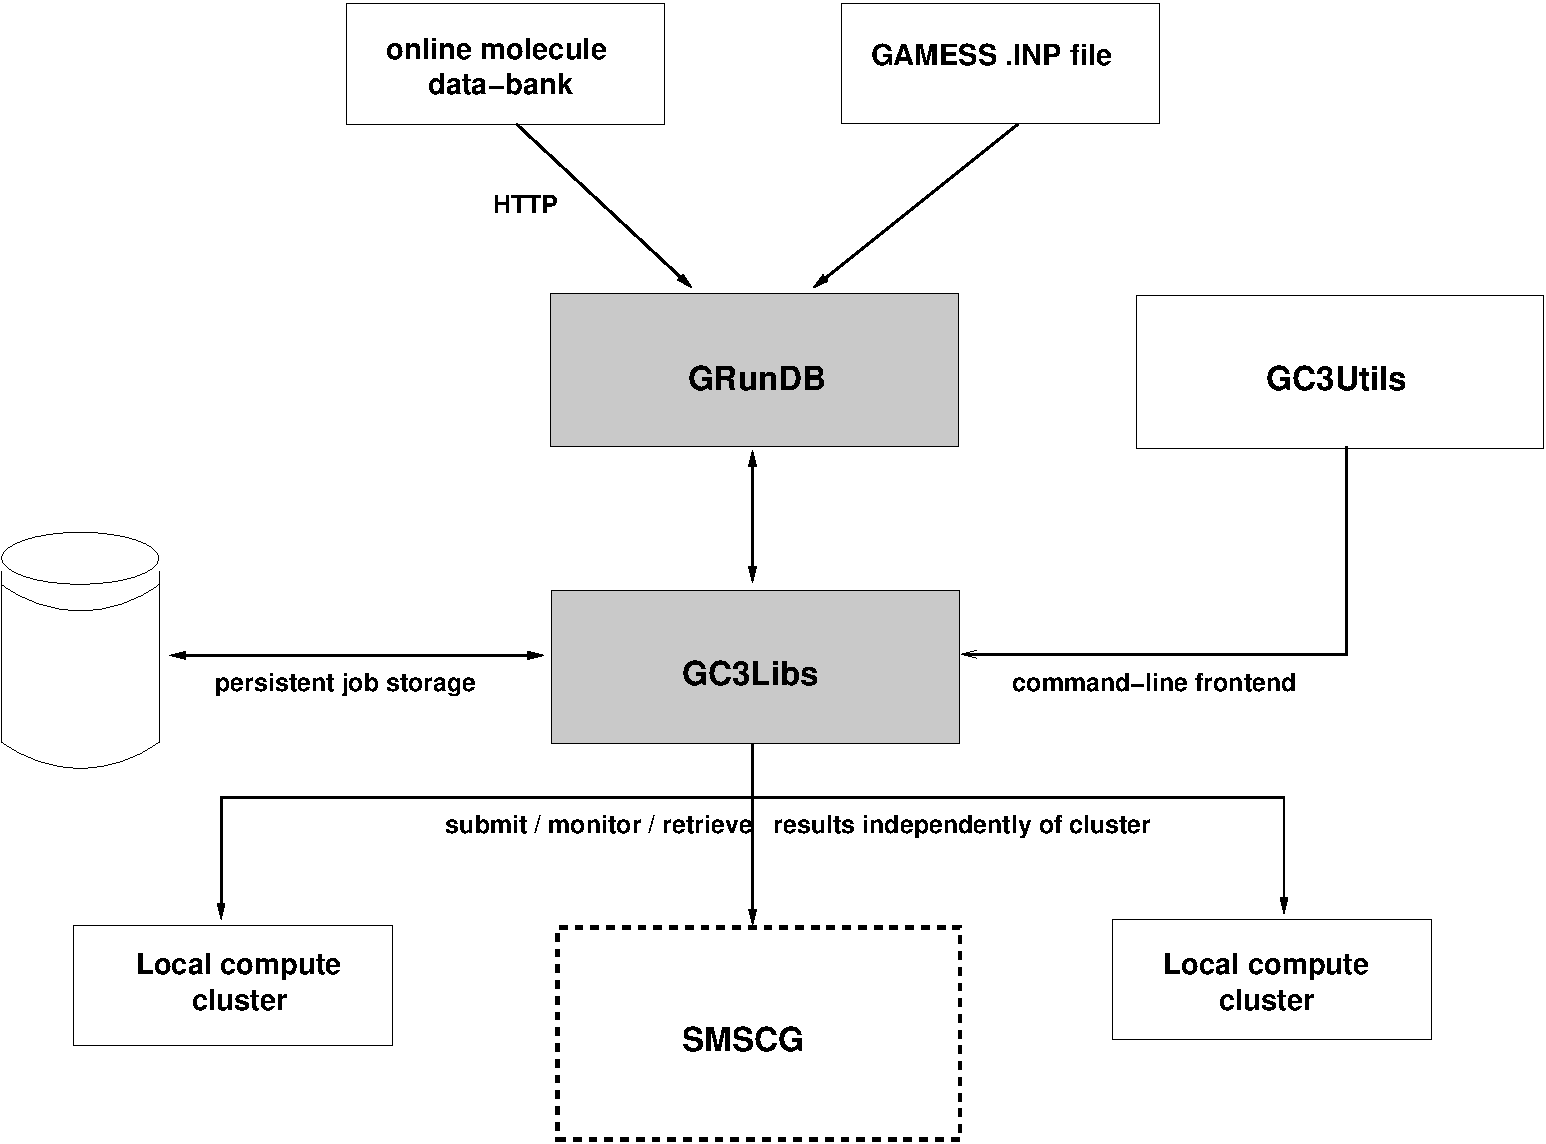
\includegraphics[width=0.8\textwidth]{architecture}
  \end{center}
\end{frame}

\begin{frame}
  \frametitle{The GC3Libs framework}

  GC3Libs is a set of Python classes to submit and control batch jobs
  to clusters and grid resources.

  \+ GC3Libs takes care of the job processing and computational
  resource control; GRunDB does the pre- and post-processing.

  \+ GC3Libs has an \emph{application-oriented} paradigm: each
  application has its own specialized job class, that knows how to
  cope with \emph{that} application's own features.

  \+
  \begin{tiny}
    Find out more at: \url{http://gc3pie.googlecode.com/}
  \end{tiny}
\end{frame}

\begin{frame}
  \frametitle{The GAMESS.UZH molecule database: Subset index}
  \begin{center}
    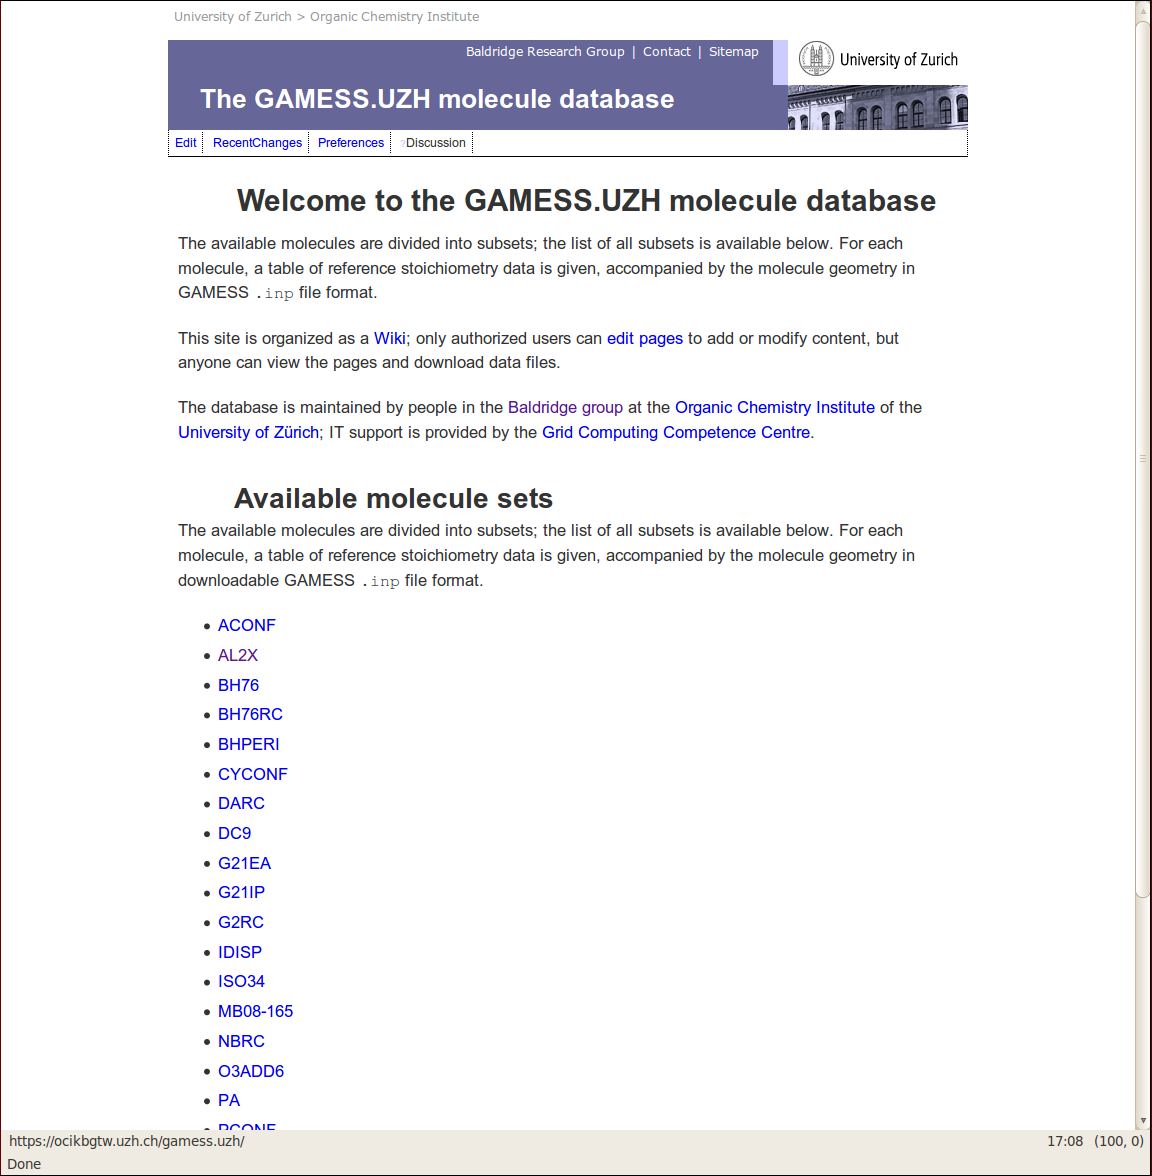
\includegraphics[height=0.9\textheight]{gamess-uzh-1}
  \end{center}
\end{frame}

\begin{frame}
  \frametitle{The GAMESS.UZH molecule database: The AL2X subset}
  \begin{center}
    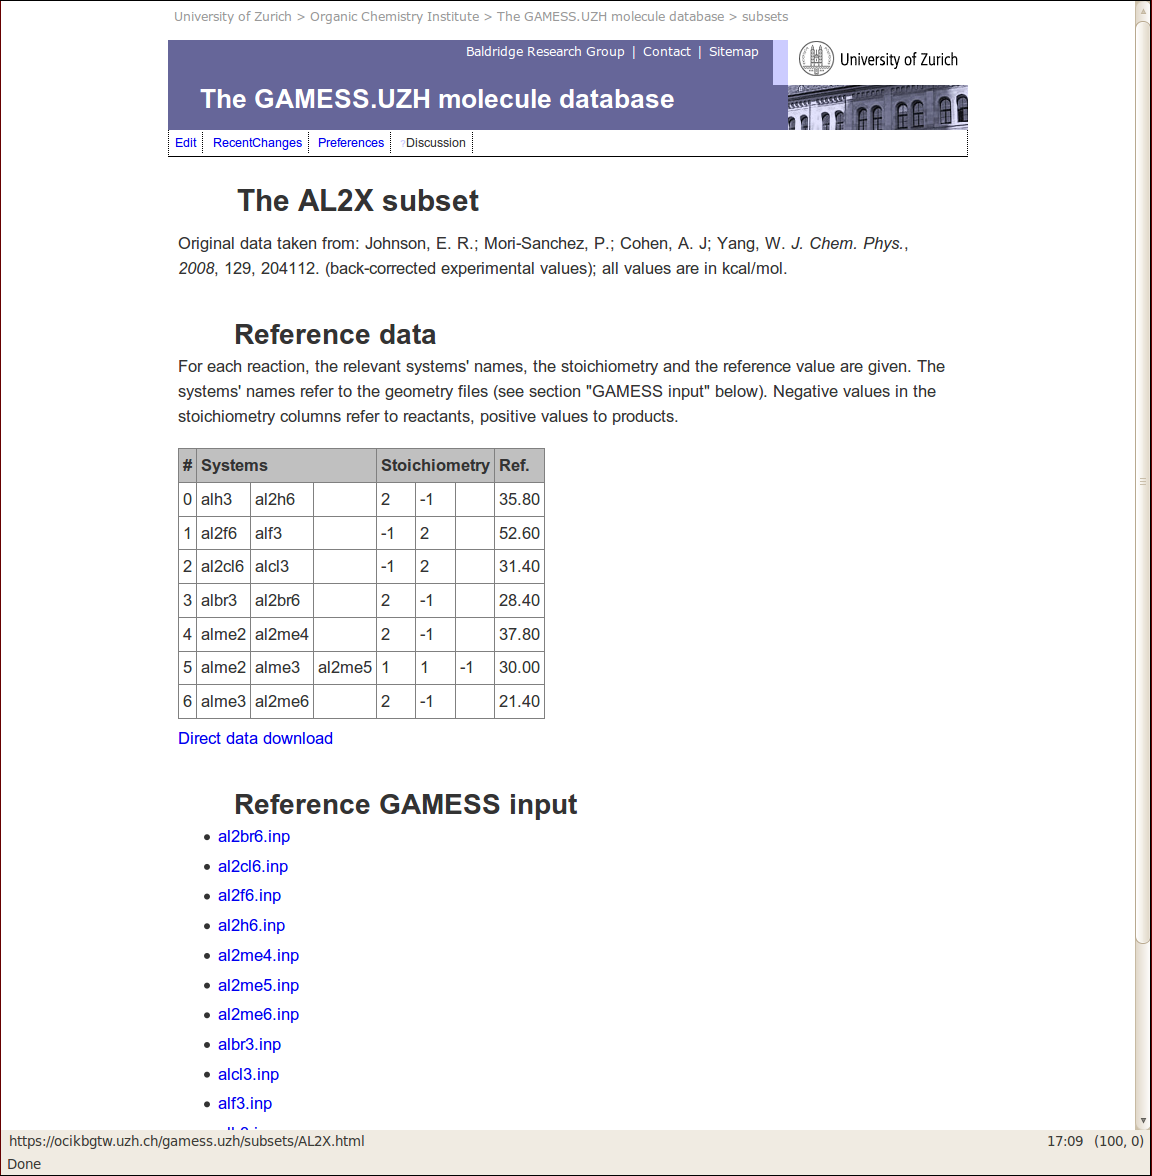
\includegraphics[height=0.9\textheight]{gamess-uzh-2}
  \end{center}
\end{frame}


\section{A demo session}

\begin{frame}[fragile]
  \frametitle{Start analysis of a molecule set}

  GRunDB creates a job for each molecule in the specified subset.
  A \emph{session} name must be given to record the current analysis.

  \+ 
  Subsets can be specified by their name on the web page.  More
  than one (or \emph{ALL}) can be analyzed in a single GRunDB go.

  \+
  \begin{footnotesize}
\begin{semiverbatim}
\$ {\bf ./grundb.py new AL2X session1}
Input file name  State (JobID)       Info
==============================================================================
al2br6           NEW (job.680)       New at Mon Nov 29 14:06:46 2010
al2cl6           NEW (job.681)       New at Mon Nov 29 14:06:46 2010
al2f6            NEW (job.682)       New at Mon Nov 29 14:06:46 2010
al2h6            NEW (job.683)       New at Mon Nov 29 14:06:46 2010
{\em ...}
alf3             NEW (job.689)       New at Mon Nov 29 14:06:47 2010
alh3             NEW (job.690)       New at Mon Nov 29 14:06:47 2010
alme2            NEW (job.691)       New at Mon Nov 29 14:06:47 2010
alme3            NEW (job.692)       New at Mon Nov 29 14:06:47 2010
\end{semiverbatim}    
  \end{footnotesize}
\end{frame}

\begin{frame}[fragile]
  \frametitle{Submit jobs to the Grid}

  Once a session has been created, a single command invocation is
  needed to submit jobs to SMSCG or University clusters.
  \+
  \begin{footnotesize}
\begin{semiverbatim}
\$ {\bf ./grundb.py progress session1}
Insert AAI/Switch password for user  m1058036 :
Queue selected: all.q@idgc3grid01.uzh.ch
File uploaded: /tmp/rmurri/rsl.qOp5wn
File uploaded: /home/rmurri/gc3/gc3utils/0.10/grundb/take1.inp.d/AL2X/al2f6.inp
  {\em ...}
Input file name  State (JobID)       Info
==============================================================================
al2br6           SUBMITTED (job.680)  Submitted at Mon Nov 29 14:08:04 2010
al2cl6           SUBMITTED (job.681)  Submitted at Mon Nov 29 14:07:53 2010
al2f6            SUBMITTED (job.682)  Submitted at Mon Nov 29 14:07:29 2010
al2h6            SUBMITTED (job.683)  Submitted at Mon Nov 29 14:07:41 2010
  {\em ...}
alh3             SUBMITTED (job.690)  Submitted at Mon Nov 29 14:07:50 2010
alme2            SUBMITTED (job.691)  Submitted at Mon Nov 29 14:07:59 2010
alme3            SUBMITTED (job.692)  Submitted at Mon Nov 29 14:08:02 2010
\end{semiverbatim}    
  \end{footnotesize}
\end{frame}

\begin{frame}[fragile]
  \frametitle{Monitor job progress and execution}

  The same command is used to monitor job execution.  This makes it
  easy to use any periodic command scheduler to carry out the task.
  \+
  \begin{footnotesize}
\begin{semiverbatim}
\$ {\bf ./grundb.py progress session1}
Input file name  State (JobID)       Info
==============================================================================
al2br6           SUBMITTED (job.680)  Submitted at Mon Nov 29 14:08:04 2010
al2cl6           RUNNING (job.681)   Running at Mon Nov 29 14:08:40 2010
al2f6            RUNNING (job.682)   Running at Mon Nov 29 14:08:40 2010
al2h6            RUNNING (job.683)   Running at Mon Nov 29 14:08:40 2010
  {\em ...}
alh3             RUNNING (job.690)   Running at Mon Nov 29 14:08:40 2010
alme2            SUBMITTED (job.691)  Submitted at Mon Nov 29 14:07:59 2010
alme3            SUBMITTED (job.692)  Submitted at Mon Nov 29 14:08:02 2010
\end{semiverbatim}    
  \end{footnotesize}
\end{frame}

\begin{frame}[fragile]
  \frametitle{Output retrieval and post-processing}

  Again, \texttt{grundb progress} will automatically retrieve and
  post-process results of jobs that have finished execution,
  extracting the energy values needed to compute stoichiometry results.
  \+
  \begin{footnotesize}
\begin{semiverbatim}
\$ {\bf ./grundb.py progress session1}
File downloaded: gsiftp://idgc3grid01.uzh.ch:2811/jobs/170571291036083905502916/alme3.out
File downloaded: gsiftp://idgc3grid01.uzh.ch:2811/jobs/170571291036083905502916/alme3.dat
  {\em ...}
Input file name  State (JobID)       Info
==============================================================================
al2br6           RUNNING (job.680)   Running at Mon Nov 29 14:09:00 2010
al2cl6           RUNNING (job.681)   Running at Mon Nov 29 14:08:40 2010
al2f6            DONE (job.682)      Final-b2plyp energy= -1084.1929109480 
al2h6            DONE (job.683)      Final-b2plyp energy= -488.2225951188 
  {\em ...}
alh3             DONE (job.690)      Final-b2plyp energy= -244.0835095562 
alme2            DONE (job.691)      Final-b2plyp energy= -322.6947308201 
alme3            DONE (job.692)      Final-b2plyp energy= -361.9996423212 
\end{semiverbatim}    
  \end{footnotesize}
\end{frame}

\begin{frame}[fragile]
  \frametitle{Interoperability / 1}

  All the data related to the jobs created by GRunDB is stored on the
  filesystem.  This is a design decision: users must retain full
  control of the data and be able to inspect every sibngle job.

  \+
  \begin{description}
  \item[{\em session}.csv]
    This is where job IDs and their statuses are recorded.  It's the
    same information you see on the video, but it can be imported into
    a spreadsheet.
  \item[{\em session}.inp.d]
    Input files for all GAMESS jobs, named after the molecule they
    represent.  Can be edited, and then resubmit the job.
  \item[{\em session}.out.d] 
    Output and error files from a job; this is the place to inspect if
    something has gone wrong, or if you want to read the full log file
    of the computations.
  \end{description}
\end{frame}

\begin{frame}[fragile]
  \frametitle{Interoperability / 2}
  
  GRunDB creates jobs and stores them using GC3Libs mechanisms, so you
  can operate on jobs with the GC3Utils command-line tools as well.

  \+ 
  Using GC3Utils allows for operations on a single job:
  \begin{itemize}
  \item What's the running status of the largest job of all? 
    \begin{itemize}\item[$\rightarrow$\space] 
      Use the \texttt{gstat} command.
    \end{itemize}
  \item Why is this molecule taking so long to compute?
    \begin{itemize}\item[$\rightarrow$\space] 
      Use the \texttt{gtail} command to peek at the output/error log.
    \end{itemize}
  \item Oops! I need to change parameters for one molecule only.
    \begin{itemize}\item[$\rightarrow$\space] 
      Use the \texttt{gresub} command to re-start a job from the
      beginning.
    \end{itemize}
  \end{itemize}
\end{frame}

\begin{frame}[fragile]
  \frametitle{Finally...}

  When all jobs are done, GRunDB computes stoichiometry data and
  compares it to the reference data.

  \begin{scriptsize}
\begin{semiverbatim}
\$ {\bf ./grundb.py progress session1}
Input file name  State (JobID)       Info
==============================================================================
al2br6           DONE (job.682)      Final r-m06 energy is -15929.9575541891
  {\em ...}                                                     after 19 iterations 
alme3            DONE (job.694)      Final r-m06 energy is -362.1226427375
                                                           after 18 iterations 
STOICHIOMETRY DATA
Reaction                            Comp. energy  (Ref. data; deviation)
==============================================================================
                                     AL2X
------------------------------------------------------------------------------
2*alh3 + -1*al2h6                         +35.70  (+35.80; -0.10)
-1*al2f6 + 2*alf3                         +48.46  (+52.60; -4.14)
-1*al2cl6 + 2*alcl3                       +28.15  (+31.40; -3.25)
2*albr3 + -1*al2br6                       +25.41  (+28.40; -2.99)
2*alme2 + -1*al2me4                       +34.52  (+37.80; -3.28)
1*alme2 + 1*alme3 + -1*al2me5             +28.55  (+30.00; -1.45)
2*alme3 + -1*al2me6                       +21.72  (+21.40; +0.32)
\end{semiverbatim}    
  \end{scriptsize}
\end{frame}

\begin{frame}
  \begin{center}
    {\Huge Thank you!}
    \\
    \+
    {\Large (Any questions?)}
  \end{center}
\end{frame}

\section{More information}

\begin{frame}
  \frametitle{References}
  \begin{small}
    \begin{description}
    \item[GRunDB]
      \url{http://gc3pie.googlecode.com/svn/branches/0.10/grundb}
    \item[GC3Libs] \url{http://gc3pie.googlecode.com/}
    \item[GAMESS(US)] \url{http://www.msg.chem.iastate.edu/gamess/}

      \begin{footnotesize}
        \+ ``General Atomic and Molecular Electronic Structure
        System'', M.~W.~Schmidt, K.~K.~Baldridge, J.~A.~Boatz,
        S.~T.~Elbert, M.~S.~Gordon, J.~H.~Jensen, S.~Koseki,
        N.~Matsunaga, K.~A.~Nguyen, S.~Su, T.~L.~Windus, M.~Dupuis,
        J.~A.~Montgomery, \emph{J. Comput. Chem.}, 14,
        1347-1363(1993).

        \+ ``Advances in electronic structure theory: GAMESS a decade
        later'', M.~S.~Gordon, M.~W.~Schmidt, pp. 1167-1189, in {\em
          Theory and Applications of Computational Chemistry: the
          first forty years}, C.~E.~Dykstra, G.~Frenking, K.~S.~Kim,
        G.~E.~Scuseria (editors), Elsevier, Amsterdam, 2005.
      \end{footnotesize}
    \end{description}
  \end{small}
\end{frame}

\begin{frame}
  \frametitle{Well, and the errors...?}

  Errors happen, and it's not necessarily a users' fault.  (e.g., disk
  full on a remote cluster)

  \+ How does GRunDB deal with this?

  \pause
  \+ Use GC3Utils to get control over the \emph{individual} job:
  \begin{itemize}
  \item Inspect job output and logs in the \emph{session.out.d}
    directory (or use the \texttt{gtail} command)
  \item Take measures against the failure
  \item Re-submit the failed job with \texttt{gresub}
  \item GRunDB will notice and re-process the results when the new job
    is done.    
  \end{itemize}

\end{frame}

\end{document}

%%% Local Variables: 
%%% mode: latex
%%% TeX-master: t
%%% x-symbol-8bits: nil
%%% End: 
